\chapter{Architecture du projet}

	\section{Arborescence du projet}

		Notre application est organisée de la manière suivante :


		\begin{figure}[H]
			\centering
			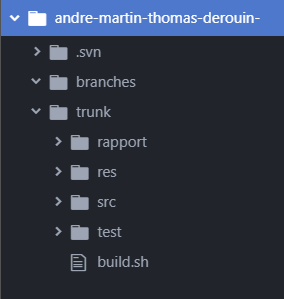
\includegraphics[width=0.5\textwidth, keepaspectratio]{img/racine.png}
		\end{figure}

		On y retrouve 4 dossiers et 1 fichier:

		\begin{description}
			\item [rapport:] contient ce rapport sous latex
			\item [res:] contient les ressources du jeu, ce qui correspond à l’image par défaut pour le taquin
			\item [src:] contient le code source de l’application
			\item [test:] contient le code se chargeant des tests unitaires
			\item [build.sh:] fichier de compilation du taquin.
		\end{description}

		Le code source du projet est situé dans le chemin \textit{src/taquin/}. Il est constitué par :

		\begin{figure}[H]
			\centering
			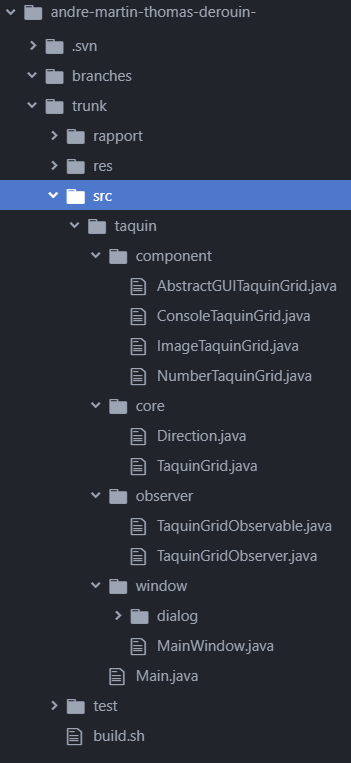
\includegraphics[width=0.5\textwidth, keepaspectratio]{img/detail.png}
		\end{figure}

		\begin{description}
			\item [component:] contient les classes des différents modes qui composent l’application.
			\item [core:] contient le cœur du jeu du taquin, qui est commun à tout les modes de jeu, ainsi que la classe qui énumère les directions
			\item [observer:] contient les classes relatives à l'implémentation du pattern Observer
			\item [window:] contient les classes permettant de gérer ce qui se rapporte à la fenêtre de jeu et des boites de dialogues
			\item [Main.java:] classe exécutable du projet.
		\end{description}

	\section{Mise en place du pattern MVC}

	Dans notre projet, il nous a été demandé d'utiliser le design pattern MVC. Ce design pattern a été mis en place de la manière suivante:

	\begin{figure}[H]
		\centering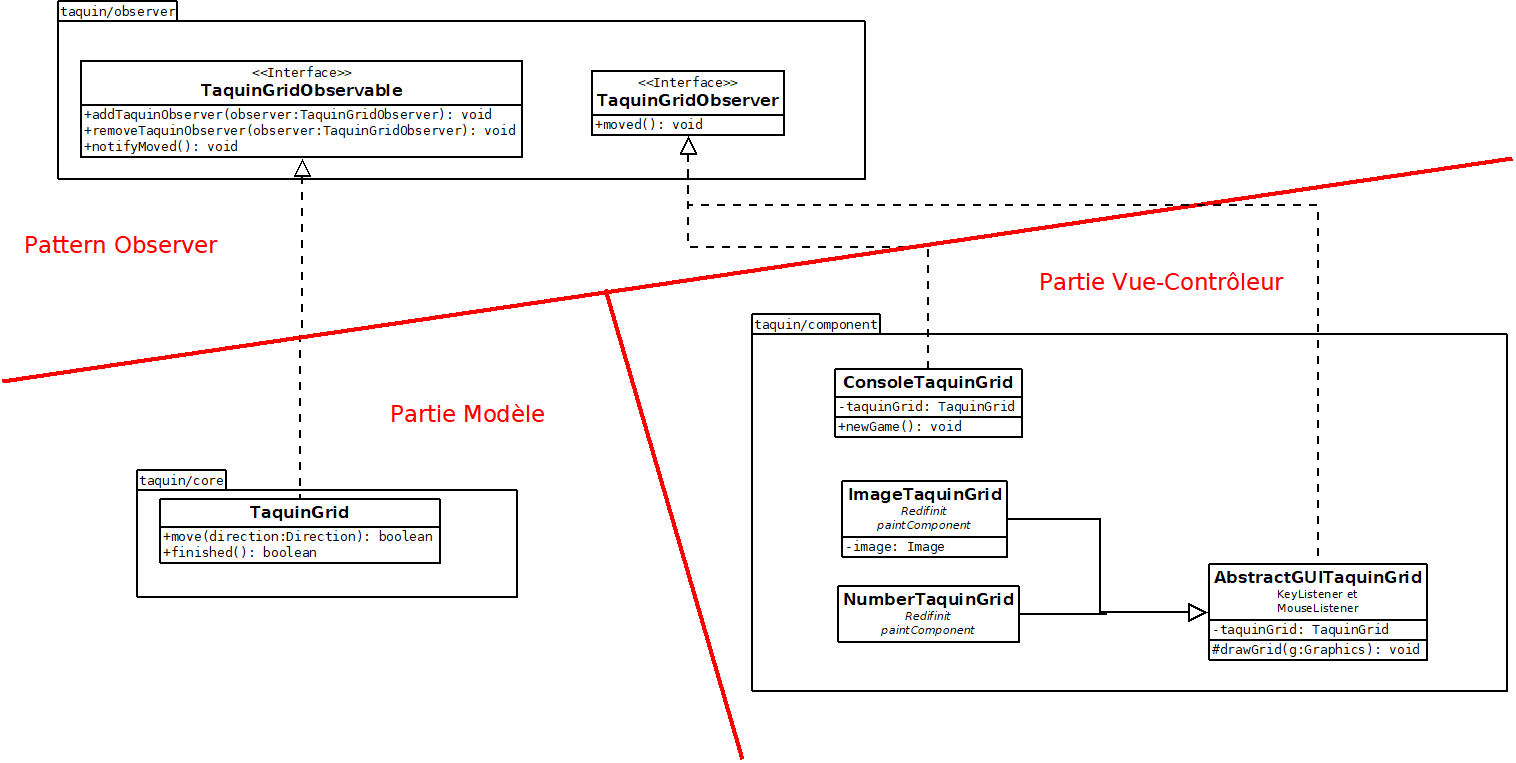
\includegraphics[width=1\textwidth, keepaspectratio]{img/diagramMVC.png}
		\caption{Notre tableau Trello}
		\label{Mise en place du M-VC}
	\end{figure}

	Nous avons la classe \textit{TaquinGrid} représente le modèle de l'application, puisqu'il s'agit du fonctionnement du taquin, donc la partie interne de l'application. Ces traitements sont absolument transparents pour l'utilisateur. Peu importe le mode d'affichage du jeu, le fonctionnement du taquin sera le même.

	Nous avons d'un autre coté, tout le package compoment, qui lui, représente à la fois les différentes vues de l'application et les contrôleurs. Dans le taquin, le modèle et le contrôleur sont intimement liés puisque un objet contrôleur pour notre taquin ne servira que pour le taquin. C'est pour cela que nous avons réalisé un couplage entre ces deux objets.

	Nous retrouvons dans le taquin trois vues-contrôleurs:


	\begin{itemize}
		\item [mode console:] vue-contrôleur représentée par la classe \textit{ConsoleTaquinGrid}
		\item [mode image:] vue-contrôleur représentée par la classe \textit{ImageTaquinGrid}
		\item [mode nombre:] vue-contrôleur représenté par la classe \textit{NumberTaquinGrid}
	\end{itemize}

	La classe mère \textit{AbstractGUITaquinGrid} n'est pas un contrôleur. Il ne s'agit que d'une vue regroupant les parties communes aux classes \textit{ImageTaquinGrid} et \textit{NumberTaquinGrid}.
